
%%%%%%%%%%%%%%%%%%%%%%% file typeinst.tex %%%%%%%%%%%%%%%%%%%%%%%%%
%
% This is the LaTeX source for the instructions to authors using
% the LaTeX document class 'llncs.cls' for contributions to
% the Lecture Notes in Computer Sciences series.
% http://www.springer.com/lncs       Springer Heidelberg 2006/05/04
%
% It may be used as a template for your own input - copy it
% to a new file with a new name and use it as the basis
% for your article.
%
% NB: the document class 'llncs' has its own and detailed documentation, see
% ftp://ftp.springer.de/data/pubftp/pub/tex/latex/llncs/latex2e/llncsdoc.pdf
%
%%%%%%%%%%%%%%%%%%%%%%%%%%%%%%%%%%%%%%%%%%%%%%%%%%%%%%%%%%%%%%%%%%%


\documentclass[runningheads,a4paper]{llncs}

\usepackage{amssymb}
\setcounter{tocdepth}{3}
\usepackage{graphicx}

\usepackage{url}
\urldef{\mailsa}\path|{alfred.hofmann, ursula.barth, ingrid.haas, frank.holzwarth,|
\urldef{\mailsb}\path|anna.kramer, leonie.kunz, christine.reiss, nicole.sator,|
\urldef{\mailsc}\path|erika.siebert-cole, peter.strasser, lncs}@springer.com|    
\newcommand{\keywords}[1]{\par\addvspace\baselineskip
\noindent\keywordname\enspace\ignorespaces#1}

\begin{document}

\mainmatter  % start of an individual contribution

% first the title is needed
\title{Discovering Bilateral and Multilateral Causal Events in GDELT}

% a short form should be given in case it is too long for the running head
\titlerunning{Lecture Notes in Computer Science: Authors' Instructions}

% the name(s) of the author(s) follow(s) next
%
% NB: Chinese authors should write their first names(s) in front of
% their surnames. This ensures that the names appear correctly in
% the running heads and the author index.
%
\author{Lei Jiang
\thanks{E-mail:lionelchange@gmail.com}%
\and Fan Mai
}
%
\authorrunning{Lecture Notes in Computer Science: Authors' Instructions}
% (feature abused for this document to repeat the title also on left hand pages)

% the affiliations are given next; don't give your e-mail address
% unless you accept that it will be published
\institute{Tapjoy Inc., San Francisco, CA 94104\\
\and 
Department of Sociology, University of Virginia \\
Charlottesville, VA 22093 USA
}

%
% NB: a more complex sample for affiliations and the mapping to the
% corresponding authors can be found in the file "llncs.dem"
% (search for the string "\mainmatter" where a contribution starts).
% "llncs.dem" accompanies the document class "llncs.cls".
%

\toctitle{Lecture Notes in Computer Science}
\tocauthor{Authors' Instructions}
\maketitle


\begin{abstract}
GDELT is one of the richest sources of event data and the hidden information could be potentially of tremendous value for its real-world reflections. While the majority of past research on these data sets puts emphasis on featured event series alone, such as Arab spring~\cite{zack2013} and violence in Afghanistan~\cite{yonamine2013}, this paper is focused on exploiting the causality between multiple types of events in different countries. In other words, for example, the actual impact of an event would result in responses from other parties, or even an escalation that more events will come thereafter. With the causal link in real-world context, time series analysis is performed on GDELT data to discover such causal links: we start from an exploration of bilateral and multilateral events in certain countries, where a strong correlation is shown; then Granger test is systematically conducted in the large-scale data set to help to identify causality in a rigorous manner. Further, with the addition of data in related parties, a scenario of prediction task is tested to show enhanced predictability as a validation of this methodology. 
\keywords{GDELT, Granger causality, bilateral events, time series analysis, prediction}
\end{abstract}

\section{Introduction}
\label{intro}

GDELT (Global Database of Events, Language and Tone)~\cite{gdelt} provides up-to-date real-world events information with its richness in covering all countries globally, providing precise geographic event information along with actor categorization and its timespan in a quarter-century (1979 to present). Preprocessing of raw events, which are from media sources, has been already done by representing all the event types and actors using a standardized code set. The abstraction actually removes much domain-specific information and thereby makes a systematic analytical methodology become available. In a high level, the GDELT data appears as spatial time series: a count can be obtained as the value at each time point for different geographic units: district, city, state or country. Based on this format, many prediction tasks can be derived, and existing work already digs into this direction: Yonamine \cite{yonamine2013} uses autoregressive integrated moving average model to make time series predictions for future levels of violence in Afghanistan districts;in ~\cite{brandt2013}, Brandt and Freeman discuss the effect of filtering GDELT time series, where the result shows filtering can't make an autoregressive fitted model better.  

Considering more attributes in the data set, event and actor types are also helpful contexts for prediction tasks. In this data challenge, we illustrate a relatively new way for predictions by utilizing auxiliary information to dig out from data. More specifically, with the time series of bilateral and multilateral event frequencies extracted, the causality between events, represented by whether one time series is useful in forecasting another (Granger causality~\cite{granger1969}), is examined between two and more parties. Using this method, the traditional time series prediction is enriched to a multivariate regression problem and the accuracy is thereby boosted.
 
In this paper, we first give an exploratory analysis to show intuitive results from GDELT data, illustrating the potential from its data in~\ref{exploration}. Then, Granger causality is formally introduced to the context and described for its application to discovering bilateral and multilateral events~\ref{granger}. After showing some interesting measurements about causal event links, we construct predictive tasks for a validation of the methodology and demonstrate our results in~\ref{results}. Lastly, we conclude the paper in~\ref{conclusion}.

\section{Event Time Series, Correlation and Causality: An Exploration}
\label{exploration}

The event time series is certainly an important piece of interest for researching GDELT data. While it is more about inter-relationship between time series in this paper, plotting the bilateral events, where the two actors represent two different countries, can give some intuitive insight. In Figure~\ref{fig:1},  left shows the relationship of event frequency between China and United States, each of which as primary actor respectively: as the blue and red curves highly overlap with each other, a strong correlation is easily seen; while correlation is bidirectional, the right interestingly shows events performed by the same primary actor, United States, but towards Japan and Korea: they share some trending as in time series, however, there are a larger amount of events for Japan at most of the time. 

\begin{figure}[!htb]
\centering
\minipage{0.50\textwidth}
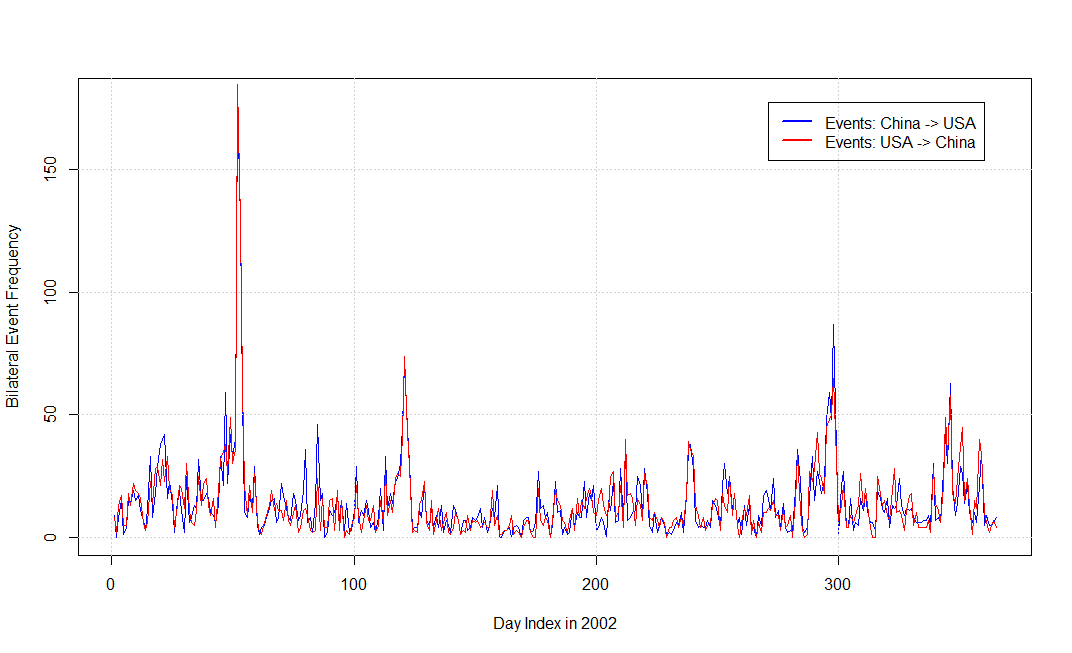
\includegraphics[width=\linewidth, height=2.2in]{sinousfreq}
\endminipage\hfill
\minipage{0.50\textwidth}
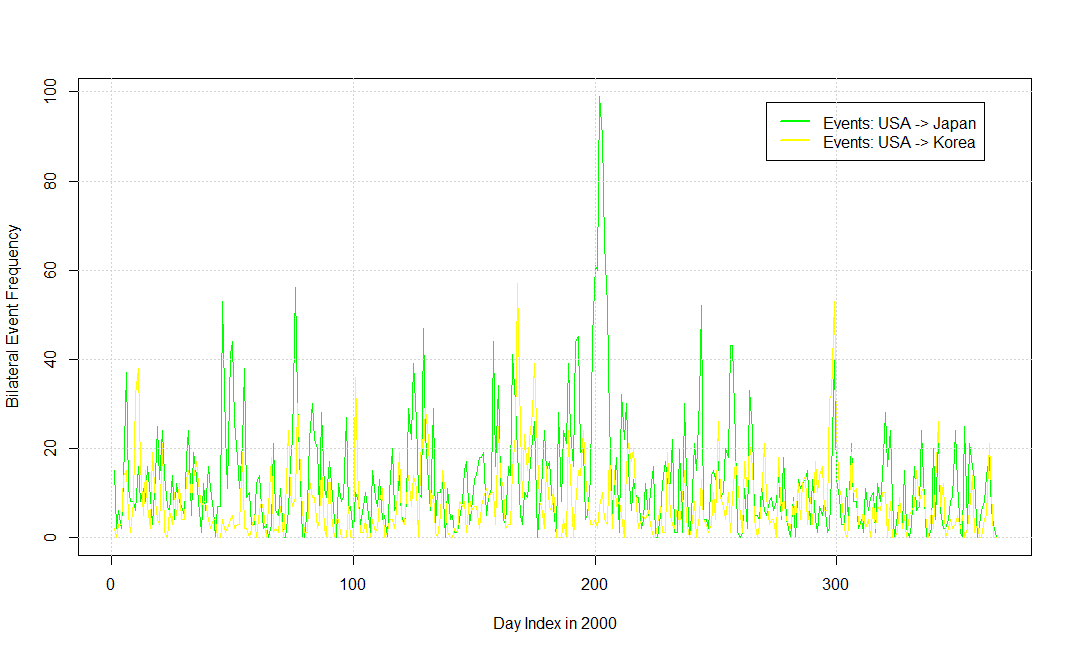
\includegraphics[width=\linewidth, height=2.2in]{usajpnkorfreq}
\endminipage\hfill
\label{fig:1}
\caption{left: The frequency of events between China and United States (each as primary actor) in 2002; right: Events acted by United States to Japan and Korea respectively in 2000}
\end{figure} 

Correlation can partly describe some features: US-China and China-US events share a high correlation coefficient (Pearson's r) 0.928, but US-Japan and US-Korea can only achieve 0.208. Within the context of correlation, a symmetric matrix can thereby derived for the frequency of events from United States to each country in Table~\ref{tab:1} (using data of 2000)

\begin{table*}
\caption{Pearson's r for US-output event frequency to the five countries}
\centering
\begin{tabular}{r c c c c c}
\hline\hline
{ } &  Brazil & China & Korea & Japan & Russia \\
\hline
Brazil  & 1.00 &  -0.0352 & -0.0488 & 0.0346 & 0.0377 \\
\hline
China  & -0.0352  & 1.00  &  0.128 &  0.0741 &  0.0826  \\
\hline
Korea  &  -0.0488  &  0.128  &  1.00  & 0.208 & 0.134  \\
\hline
Japan  &  0.0346  &  0.0741 &  0.208 &  1.00  & 0.102 \\
\hline
Russia  &  0.0377   &  0.0826 &  0.134 &  0.102  & 1.00 \\
\hline\hline
\end{tabular}
\label{tab:1}
\end{table*}

A close-to-zero correlation coefficient would not be of much help. Thus, with a question in mind: how to make use of the seemingly relationship between event frequencies and unleash the potential for predictive analysis, it brings in a unidirectional measurement: Granger causality~\cite{granger1969}. 

\section{Granger Causality for Bilateral and Multilateral Events}
\label{granger}

In a real-world global network, the diplomatic behavior between countries will make an impact in the world, sometimes especially important for  neighbor countries or those joining the same union. Thereby, there could be subsequent events from other countries. Such a chain reaction makes Granger causality explainable. Also, there exist both bilateral and multilateral events: in practical data mining, bilateral events can be discovered first, and then multilateral events are further derived as an optimization.

\subsection{Bilateral events}
Intuitively, two time series can have a link, from one to another, whenever causality can be found. In other words, one time series is helpful for forecasting the other one. Granger causality is examined towards such a statistical hypothesis: the following two equations are to be fitted and an F-test (or t-test) will go through. 

\begin{equation}
\label{eq:1}
	y_{t} = a_{1}y_{t-1}+a_{2}y_{t-2}+...+a_{i}y_{t-i}+\sigma
\end{equation} 
\begin{equation}
\label{eq:2}
	y_{t} = b_{1}y_{t-1}+b_{2}y_{t-2}+...+b_{i}y_{t-i}+b_{i+1}x_{t-m}+...+b_{i+n-m+1}x_{t-n}+\sigma
\end{equation} 

While $x$ is a variable from another time series, the level of "helpfulness'' of $x$ would determine the bivariate causality based on a computed {\em p}-value from regression-based {\em F}-value. From GDELT data, we select 15 countries  and conduct a search for pairwise {\em causal links}: with a {\em p}-value of 0.05, either "$'A->B$'' or "$B->A$'' below {\em p}-value in a Granger test is considered a link (if both values are below, the smaller one is chosen). Then, a causality-graph can be constructed based upon links. In Table~\ref{tab:2} and \ref{tab:3}), the basic connectivity analysis is conducted for both 2000 and 2001 data: an "out-degree'', for its real-world metaphor, could mean a country is an initiator for its bilateral activities, and "in-degree'' means a reaction or response contingent to the cause.

\begin{table*}
\caption{A causality-graph connectivity analysis for 2000 between 15 countries}
\centering
\begin{tabular}{r c c c c c }
\hline\hline
{} & China &  France & Russia & United Kingdom & United States   \\
\hline
Out-degree  & 4 &  4 & 5 & 5 & 5 \\
\hline
In-degree  & 6 & 5 & 8 & 4 & 5\\
\hline
{} & Japan & Korea & Germany & Brazil & North Korea \\
\hline
Out-degree &  4 & 5 & 5 & 2 & 0 \\
\hline
In-degree  & 5 & 4 & 5 & 0 & 5 \\
\hline
{}  & Afghanistan & Iran & Iraq & Saudi Arabia & Syria\\
\hline
Out-degree   & 4 & 8 & 3 & 4 & 6\\
\hline
In-degree   & 2 & 3 & 5 & 2 & 5 \\
\hline\hline
\end{tabular}
\label{tab:2}
\end{table*}

 In general, the number of degrees could represent activeness. While we don't choose to visualize the actual graph (without misleading it to real country-country relationships), it could show that from 2000 to 2001, the United States becomes more proactive (from (5,5) to (8,3), for a possible reason of the 911 tragic event, and other countries seem to be more responsive to that in 2001 (e.g. China,  United Kingdom, Korea make the transition with more in-degrees, and that doesn't affect the pattern of Iran).ƒ

\begin{table*}
\caption{A causality-graph connectivity analysis for 2001 between 15 countries}
\centering
\begin{tabular}{r c c c c c  }
\hline\hline
{} & China &  France & Russia & United Kingdom & United States   \\
\hline
Out-degree  & 5 &  3 & 5 & 1 & 8 \\
\hline
In-degree  & 8 & 6 & 7 & 8 & 3  \\
\hline
{} & Japan & Korea & Germany & Brazil & North Korea \\
\hline
Out-degree & 4 & 2 & 4   & 6 & 5 \\
\hline
In-degree & 6 & 8 & 6  & 1 & 4 \\
\hline
{}  & Afghanistan & Iran & Iraq & Saudi Arabia & Syria\\
\hline
Out-degree & 9 & 8 & 6 & 7 & 2\\
\hline
In-degree & 3 & 3 & 5 & 3 & 4 \\
\hline\hline
\end{tabular}
\label{tab:3}
\end{table*}

\subsection{Causal links and multilateral events}

Following the bilateral causal links in last subsection, the discovery is furthered to connecting more than two parties with causality. Practically, adding one more party to a combinational search scenario can add exponent-level computation complexity due to {\em the curse of dimensionality}. On the other hand, inserting more and more variables to Granger test would result in overfitting in a non-noise-free data setting. Thereby, multilateral events are considered to be an optimization from a single link of two parties.  

The search algorithm is adopted in the following routine: 
\\
\\
\textbf{Step 0}: Preprocessing raw GDELT data to extract bilateral events time series;
\\
\\
\textbf{Step 1}: Searching for causal links rooted from a certain country $X$ (with an out-degree from X) by comparing all the possible pairs $(A,B)$  such that event series "$X -> A$' and "$X -> B$' form a causal link; Then in the same way, seek for $(A,B)$ such that event series "$A -> X$'' and "$B -> X$'' could be a causal link;
\\
\\
\textbf{Step 2}:  Combining triangle relationships in pairwise causal links: e.g. "$X -> A$'' and "$X -> B$'' could be a causal link, while "$'X -> C$' and " $X -> B$'' is also a causal link; Then it is considered that both "$X -> A$'' and " $X -> C$'' can help with predicting "$ X-> B$''. 
\\
\\
It is worth noting that a multivariate Granger test for such multilateral events is conceivable. However, as the aforementioned reason about overfitting, the hypothesis testing here may not be performed in the same way as bivariate Granger test ({\em p}-value may not be comparable at this time. That is why multilateral causal links are towards a heuristic framework at this stage.

Using GDELT data ranging from 2000 to 2005, we are able to exploit all the bivariate causal links (under a rigorous framework) that cover three parties. Figure 2 shows the change. As the extracted data over the 15 countries could be considered as a sample network, where the total number of possible links remains the same all the time, the variation over years actually indicates network {\em assortativity}: when more links emerge, it means there are increasing real-world cooperations being organized and produces some well-defined network structure. For an individual country, the number of causal links could also mean the level of influence or activeness: United States and China almost both follow the global trend (United States is more active with a larger number though), but that is not the pattern of Russia.

\begin{figure}[!htb]
\label{fig:2}
\centering
%\minipage{0.80\textwidth}
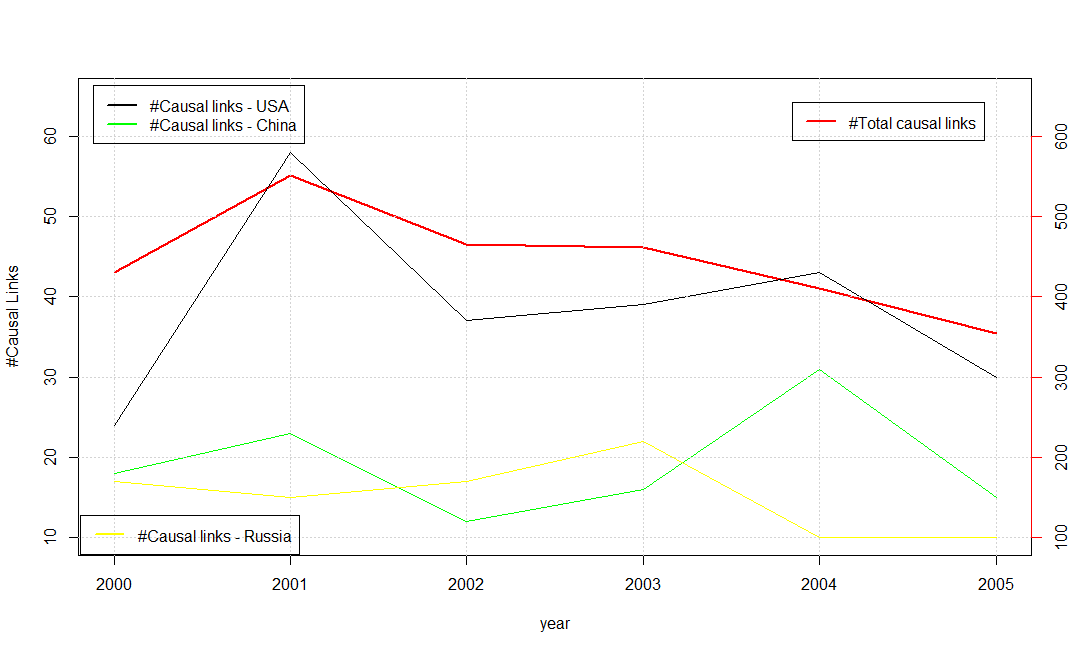
\includegraphics[width=\linewidth, height=2.2in]{causallinktrend}
%\endminipage\hfill
\caption{Trend of number of causal links in the sample network from 2000-2005}
\end{figure} 

\section{ Predictive Analysis}
\label{results}
From the perspective of data mining, the causal links are meant to serve predictive analysis, where the additional information from data could be utilized. In this section, the enhanced predictability is shown through a comparison, between traditional time series forecasting and with the help of auxiliary time series (empowered by pre-trained causal links). 

To illustrate the advantage, the 2001 data is used, where the regression task is towards the bilateral event frequency between United States and another country (United States-Afghanistan, United States-North Korea, and United States-Saudi Arabia). A linear regression is used here to fit the model: first as traditional time series prediction, it uses only the past time points (3 past time step) of the targeted time series to predict the next; then, when auxiliary time series from other countries is brought in, the corresponding time points also participate in the fitted model. Fitted {\em sum of square} (SSQ) becomes the criteria as in Table~\ref{tab:4}. 

\begin{table*}
\caption{Fitted sum of square for 2001 United States bilateral event frequency}
\centering
\begin{tabular}{r c c}
\hline\hline
{ } &  Time Series ($lag=3$) &  One auxiliary time series 1  \\
\hline
USA-AFG  & 78369.78 &  77691.52/DEU \\
\hline
{}  & One auxiliary time series 2 & Two auxiliary time series \\
\hline
USA-AFG &  77367.96/KOR  & 76883.92 \\
\hline
{ } &  Time Series ($lag=1-3$) &  One auxiliary time series 1  \\
\hline
USA-PRK  & 24314.52  & 24167.58/DEU  \\
\hline
{}  & One auxiliary time series 2 & Two auxiliary time series \\
\hline
USA-PRK  & 24124.1/KOR  &  23965.08\\
\hline
{ } &  Time Series ($lag=3$) &  One auxiliary time series 1  \\
\hline
USA-SAU  &  12890.06  &  12446.62/AFG \\
\hline
{}  & One auxiliary time series 2 & Two auxiliary time series \\
\hline
USA-SAU   &  12856.84/IRN  &  12424.87 \\
\hline
{ } &  Time Series ($lag=3$) &  One auxiliary time series 1  \\
\hline
USA-JPN  &  106580.1  & 103334.4/SAU \\
\hline
{}  & One auxiliary time series 2 & Two auxiliary time series \\
\hline
USA-JPN &  103288.2/PRK  & 100050.2 \\
\hline\hline
\end{tabular}
\label{tab:4}
\end{table*}

In each case , the listed two countries, as in column "One auxiliary time series 1' and "One auxiliary time series 2'', are both used for the scenario of "Two auxiliary time series". Such auxiliaries, except the last one of predicting USA-Japan, all appear in multilateral causal links, identified to be helpful for the prediction task.  For the last case, auxiliaries appear as the other side of causality link (in-degree), but still gain a positive effect. 


\section{Conclusion and Future Work}
\label{conclusion}
In this paper, we illustrate our insight for the GDELT database through a broad range of analysis, including exploratory analysis, Granger causality test, searching for pattern and predictive analysis. The current results show that the causal links hidden in data set, with a real-world metaphor of bilateral and multilateral causal events, could have a profound effect in deeply analyzing the activities and trends over different countries of the world. While the authors is new to GDELT data set via the data  challenge, there are the following conceivable directions for future work: {\em i)} Using event type information to construct finer-level models; and {\em ii)} Developing larger-scale macine learning pipeline to construct rigorous model with iterative tuning. All the related source code (in R and Python) for this data challenge is available\footnotemark[1].

\footnotetext[1]{https://github.com/lionelc/GDELT\_SBP2014\_data\_challenge}


\begin{thebibliography}{1}
\bibitem{gdelt} Leetaru, Kalev and Schrodt, Philip, "GDELT: Global Data on Events, Language, and Tone, 1979-2012'' in {\em International Studies Association Annual Conference}, April 2013. San Diego, CA.
\bibitem{zack2013} Z. Steinert-Threlkeld, "The Arab spring and GDELT'', posted at http://blog.gdelt.org/2013/10/02/the-arab-spring-and-gdelt/ , accessed on Jan 11, 2014.
\bibitem{yonamine2013} J.E. Yonamine, "Predicting future levels of violence in Afghanistan districts using GDELT, ''  published at http://gdelt.utdallas.edu/data/papers/Predicting\_Future\_Levels\_of\_Violence\_in\_Afghanistan
\_Districts\_using\_GDELT.pdf , accessed on Jan 10, 2014.
\bibitem{brandt2013} P.T. Brandt and J.R. Freeman, "Why (Not to) Filter or Pre-Whiten the GDELT Time Series?, '' published at http://www.utdallas.edu/\~pbrandt/Patrick\_Brandts\_Website/Research\_files/WhyFilterGDELT.pdf . Accessed on Jan 10, 2014. 
\bibitem{granger1969} C.W.J. Granger, "Investigating causal relations by econometric models and cross-spectral methods," {\em Econometrica}, 37(3) pp. 424-438.


\end{thebibliography}


\end{document}
